% !TeX program = pdflatex
% !BIB program = bibtex
% Template LaTeX file for DAFx-19 papers
%
% To generate the correct references using BibTeX, run
%     latex, bibtex, latex, latex
% modified...
% - from DAFx-00 to DAFx-02 by Florian Keiler, 2002-07-08
% - from DAFx-02 to DAFx-03 by Gianpaolo Evangelista
% - from DAFx-05 to DAFx-06 by Vincent Verfaille, 2006-02-05
% - from DAFx-06 to DAFx-07 by Vincent Verfaille, 2007-01-05
%                          and Sylvain Marchand, 2007-01-31
% - from DAFx-07 to DAFx-08 by Henri Penttinen, 2007-12-12
%                          and Jyri Pakarinen 2008-01-28
% - from DAFx-08 to DAFx-09 by Giorgio Prandi, Fabio Antonacci 2008-10-03
% - from DAFx-09 to DAFx-10 by Hannes Pomberger 2010-02-01
% - from DAFx-10 to DAFx-12 by Jez Wells 2011
% - from DAFx-12 to DAFx-14 by Sascha Disch 2013
% - from DAFx-15 to DAFx-16 by Pavel Rajmic 2015
% - from DAFx-16 to DAFx-17 by Brian Hamilton 2016
% - from DAFx-18 to DAFx-19 by Dave Moffat 2019
%
% Template with hyper-references (links) active after conversion to pdf
% (with the distiller) or if compiled with pdflatex.
%
% 20060205: added package 'hypcap' to correct hyperlinks to figures and tables
%                      use of \papertitle and \paperauthorA, etc for same title in PDF and Metadata
%
% 1) Please compile using latex or pdflatex.
% 2) If using pdflatex, you need your figures in a file format other than eps! e.g. png or jpg is working
% 3) Please use "paperftitle" and "pdfauthor" definitions below

%------------------------------------------------------------------------------------------
%  !  !  !  !  !  !  !  !  !  !  !  ! user defined variables  !  !  !  !  !  !  !  !  !  !  !  !  !  !
% Please use these commands to define title and author(s) of the paper:
\def\papertitle{A Stable Structure for Nonlinear Biquad Filters}
\def\paperauthorA{Jatin Chowdhury}

% Authors' affiliations have to be set below

%------------------------------------------------------------------------------------------
\documentclass[twoside,a4paper]{article}
\usepackage{dafx_19}
\usepackage{amsmath,amssymb,amsfonts,amsthm}
\usepackage{euscript}
\usepackage[latin1]{inputenc}
\usepackage[T1]{fontenc}
\usepackage{ifpdf}

\usepackage[english]{babel}
\usepackage{caption}
\usepackage{subfig} % or can use subcaption package
\usepackage{xcolor}

\setcounter{page}{1}
\ninept

\usepackage{times}
% Saves a lot of ouptut space in PDF... after conversion with the distiller
% Delete if you cannot get PS fonts working on your system.

% pdf-tex settings: detect automatically if run by latex or pdflatex
\newif\ifpdf
\ifx\pdfoutput\relax
\else
   \ifcase\pdfoutput
      \pdffalse
   \else
      \pdftrue
\fi

\ifpdf % compiling with pdflatex
  \usepackage[pdftex,
    pdftitle={\papertitle},
    pdfauthor={\paperauthorA},
    colorlinks=false, % links are activated as colror boxes instead of color text
    bookmarksnumbered, % use section numbers with bookmarks
    pdfstartview=XYZ % start with zoom=100% instead of full screen; especially useful if working with a big screen :-)
  ]{hyperref}
  \pdfcompresslevel=9
  \usepackage[pdftex]{graphicx}
  \usepackage[figure,table]{hypcap}
\else % compiling with latex
  \usepackage[dvips]{epsfig,graphicx}
  \usepackage[dvips,
    colorlinks=false, % no color links
    bookmarksnumbered, % use section numbers with bookmarks
    pdfstartview=XYZ % start with zoom=100% instead of full screen
  ]{hyperref}
  % hyperrefs are active in the pdf file after conversion
  \usepackage[figure,table]{hypcap}
\fi

% My packages
\usepackage{cleveref}
\usepackage{tikz}
\usetikzlibrary{dsp,chains}
\usepackage{tkz-euclide}
\usetkzobj{all}

\usepackage{listings}
\definecolor{codegreen}{rgb}{0,0.6,0}
\definecolor{codegray}{rgb}{0.5,0.5,0.5}
\definecolor{codepurple}{rgb}{0.58,0,0.82}
\definecolor{backcolour}{rgb}{0.95,0.95,0.92}
 
\lstdefinestyle{mystyle}{
    backgroundcolor=\color{backcolour},   
    commentstyle=\color{codegreen},
    keywordstyle=\color{magenta},
    numberstyle=\tiny\color{codegray},
    stringstyle=\color{codepurple},
    basicstyle=\footnotesize,
    columns=flexible,
    breakatwhitespace=false,         
    breaklines=true,                 
    captionpos=b,                    
    keepspaces=true,                               
    showspaces=false,                
    showstringspaces=false,
    showtabs=false,                  
    tabsize=4
}
 
\lstset{style=mystyle}

\DeclareMathAlphabet{\mathpzc}{OT1}{pzc}{m}{it}
\newcommand{\z}{\mathpzc{z}}

\title{\papertitle}

\affiliation{
\paperauthorA \,}
{\href{http://ccrma.stanford.edu}{Center for Computer Research in Music and Acoustics} \\ Stanford University \\ Palo Alto, CA \\ {\tt \href{mailto:jatin@ccrma.stanford.edu}{jatin@ccrma.stanford.edu}}}

\begin{document}
% more pdf-tex settings:
\ifpdf % used graphic file format for pdflatex
  \DeclareGraphicsExtensions{.png,.jpg,.pdf}
\else  % used graphic file format for latex
  \DeclareGraphicsExtensions{.eps}
\fi

\maketitle

\begin{abstract}
Biquad filters are a common tool for filter design. In this
writing, we develop a structure for creating nonlinear biquad
filters with guaranteed stability. We examine an example filter
designed with this structure, and compare to a corresponding
analog filter.
\end{abstract}

\section{Introduction}
A ``biquad'' filter refers to a general 2nd order IIR filter.
In digital signal processing, biquad filters are often useful
since any higher-order filter can be implemented using a cascade
of biquad filters. While digital biquad filters are typically implemented
as linear processors, for audio applications it can be useful to
implement nonlinear filters. For example, in \cite{SKF} the authors
use a passive model of operational amplifiers to model the nonlinear
behaviour of a Sallen-Key lowpass filter. In this writing, we strive
to develop a more general nonlinear filter structure, one that can be
used for analog modelling, but does not necessarily depend on analog
modelling principles to be understood and implemented.

\section{Developing the Structure}
\subsection{Linear Filter}
%
We begin with the equation for a biquad filter:
%
\begin{equation}
\begin{split}
    y[n] = b_0 u[n] + b_1 u[n-1] + b_2 u[n-2] \\ - a_1 y[n-1] - a_2 y[n-2]
\end{split}
    \label{eq:bq}
\end{equation}
%
Where $y$ is the output signal, $u$ is the input signal, and $a_n$ and $b_n$
are the feed-back and feed-forward filter coefficients, respectively.
There are several convenient "direct forms" for implementing biquad filters.
In this writing we will focus on the ``Transposed Direct Form II'' (TDF-II),
which is popular for its numerical properties \cite{JOSFilters}.
%
\begin{figure}[ht]
    \center
    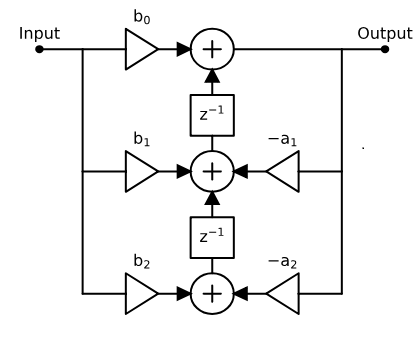
\includegraphics[width=2.3in]{../Pics/TDF-II-White.png}
    \caption{\label{TDF-II}{\it Transposed Direct Form II}}
\end{figure}
%
Note that the poles of the filter can be described using the quadratic
equation.
\begin{equation}
    p = \frac{-a_1 \pm \sqrt{a_1^2- 4a_2}}{2}
    \label{eq:poles_lin}
\end{equation}
%

\subsection{Nonlinear Elements}
%
We now propose adding nonlinear elements to the above filter structure.
We will refer to these nonlinear elements as ``base nonlinearities''
To keep the discussion as broad as possible, we consider any one-to-one
nonlinear function $f_{NL}(x)$. It will often be convenient to consider
the input-dependent ``gain'' of the nonlinear function:
%
\begin{equation}
    g_{NL}(x) = \frac{f_{NL}(x)}{x}
    \label{eq:g_NL}
\end{equation}
%
In order to maintain stability, we propose the following constraint on
any nonlinear functions used in these filters:
%
\begin{equation}
    0 \leq g_{NL}(x)\leq 1
    \label{eq:NL_constraint}
\end{equation}
%
Many musical nonlinearities satisfy this constraint, including most
saturating, dropout, and half-wave rectifying nonlinearities.
Of particular interest to us will be saturating nonlinearities,
including hard-clippers, soft-clippers, and sigmoid-like functions
(see \cref{Sats}).
Saturating nonlinearities satisfy the property that
%
\begin{equation}
    |x| \rightarrow \infty, \ g_{sat}(x) \rightarrow 0
    \label{eq:Sat_constraint}
\end{equation}
%
\begin{figure}[ht]
    \center
    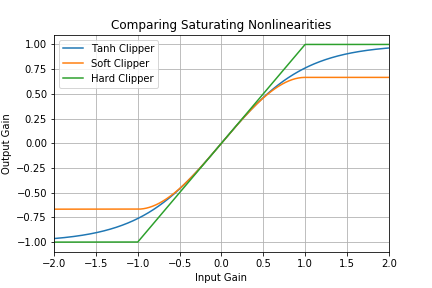
\includegraphics[width=3in]{../Pics/Sat-NLs.png}
    \caption{\label{Sats}{\it Saturating Nonlinearities}}
\end{figure}
%

\subsection{Nonlinear Filter Structure}
%
We now propose adding nonlinear elements to the TDF-II strcuture in the
following fashion (see \cref{NL-TDF-II}).
%
\begin{figure}[ht]
    \center
    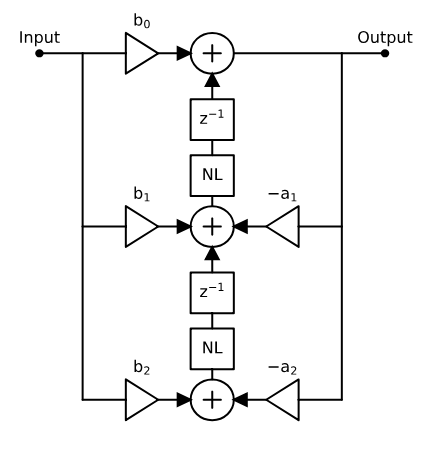
\includegraphics[width=2.3in]{../Pics/NL-TDF-II-White.png}
    \caption{\label{NL-TDF-II}{\it Nonlinear Transposed Direct Form II.
                                The ``NL'' blocks refer to a generalized
                                nonlinear element.}}
\end{figure}
%
The equation for the nonlinear biquad filter then becomes:
%
\begin{equation}
\begin{split}
    y[n] = b_0 u[n]
         + f_{NL} (b_1 u[n-1] - a_1 y[n-1] \\
         + f_{NL} (b_2 u[n-2] - a_2 y[n-2]))
\end{split}
    \label{eq:bq_NL}
\end{equation}
%
Here it can be useful to define filter ``state variables''
%
\begin{equation}
\begin{split}
    x_1 = f_{NL} (x_2) + b_1 u[n-1] - a_1 y[n-1] \\
    x_2 = b_2 u[n-2] - a_2 y[n-2]
\end{split}
    \label{eq:states}
\end{equation}
%
Note that for saturating base nonlinearities, as the input $u$ grows large,
the other terms will become negigible.
\newline\newline
Now we can replace the nonlinear elements with their input-dependent gains:
%
\begin{equation}
\begin{split}
    g_1 =  \frac{f_{NL}(x_1)}{x_1} \\
    g_2 =  \frac{f_{NL}(x_2)}{x_2}
\end{split}
    \label{eq:gs}
\end{equation}
%
Then \cref{eq:bq_NL} can be re-written:
%
\begin{equation}
\begin{split}
    y[n] = b_0 u[n]
         + g_1 (b_1 u[n-1] - a_1 y[n-1] \\
         + g_2 (b_2 u[n-2] - a_2 y[n-2]))
\end{split}
    \label{eq:bq_re-write}
\end{equation}
%
Finally, we can re-write the filter coefficients as variables dependent on
state variables:
%
\begin{align}
\begin{split}
    b_0' &= b_0\\
    b_1' &= g_1 b_1\\
    b_2' &= g_1 g_2 b_2\\
    a_1' &= g_1 a_1\\
    a_2' &= g_1 g_2 a_2
\end{split}
    \label{eq:bq_coefs_re-write}
\end{align}
%
\begin{equation}
\begin{split}
    y'[n] = b_0' u[n]
    + b_1' u[n-1] - a_1' y[n-1] \\
    + b_2' u[n-2] - a_2' y[n-2]
\end{split}
    \label{eq:bq_re-write2}
\end{equation}
%

\subsection{Guaranteed Stability}
%
Since the coefficients of the biquad filter will be dependent on the
state of the filter, the instantaneous poles of the filter will be
dependent as well. In order to calculate the instantaneous poles of
the nonlinear biquad structure, we can adjust the formula from
\cref{eq:poles_lin}.
%
\begin{equation}
    p = \frac{-g_1 a_1 \pm \sqrt{g_l^2 a_1^2- 4 g_1 g_2 a_2}}{2}
    \label{eq:poles_nl}
\end{equation}
%
From the constraint in \cref{eq:NL_constraint}, we can see that the
magnitude of the instantaneous pole will always be less than or equal to
the magnitude of the original pole from the corresponding linear filter.
Therefore, we know that any nonlinear biquad filter designed with the above
structure will be stable provided that the corresponding linear filter is
stable, and that the constraint from \cref{eq:NL_constraint} is satisfied.
\newline\newline
For saturating base nonlinearities, we can see from \cref{eq:Sat_constraint}
that as the state variables grow large, the poles will go to zero.

\section{Example: Resonant Lowpass Filter}

As an example of the nonlinear biquad structure developed in the
previous section, we will now examine a resonant lowpass filter
designed with the nonlinear structure, and compare to a corresponding
analog filter.

\subsection{Digital Nonlinear Filter}

Our example filter will be a lowpass filter with a cutoff frequency at
$f_c = 1\text{ kHz}$, and $Q = 10$. For our nonlinear elements we will
use a hyperbolic tangent function $f_{NL}(x) = \tanh (x)$. Note that
this nonlinear function belongs to the class of saturating nonlinearities
described by \cref{eq:Sat_constraint}.
\newline\newline
In \cref{NL-LPF-freq} we show the response of this filter for sine sweeps of
various amplitudes, compared to the frequency response of the corresponding
linear filter.
%
\begin{figure}[ht]
    \center
    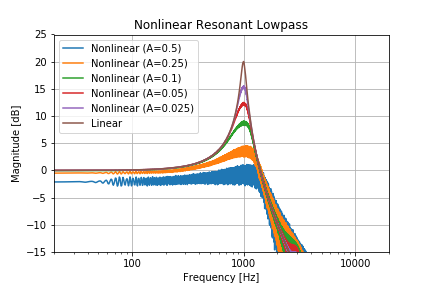
\includegraphics[width=3in]{../Pics/NL-LPF.png}
    \caption{\label{NL-LPF-freq}{\it Frequency responses of nonlinear lowpass
                                    filters at varying amplitudes.}}
\end{figure}
%
In \cref{pzPlots} we show the movement of the poles and zeros of
the filter for varying steady state inputs. We calculate the instantaneous
poles using \cref{eq:poles_nl}, using $g_1 = g_2 = g$, as described in
each figure.

\begin{figure*}[!ht]
    % \center
    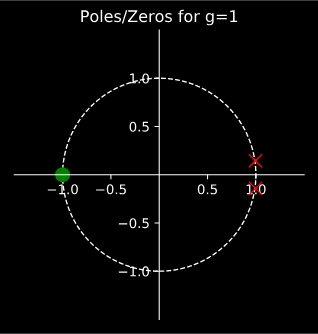
\includegraphics[width=1.7in]{../Pics/pz1.png}
    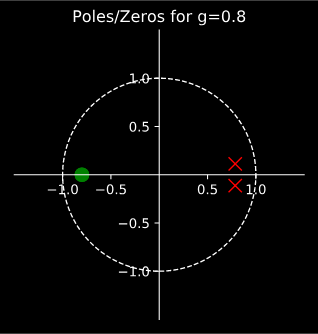
\includegraphics[width=1.7in]{../Pics/pz08.png}
    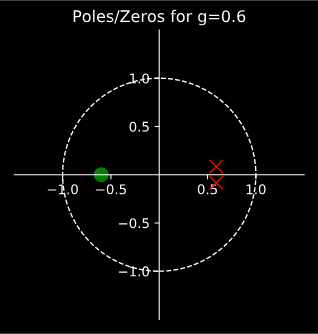
\includegraphics[width=1.7in]{../Pics/pz06.png}
    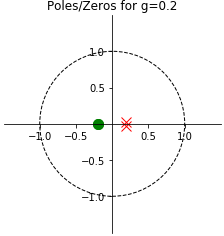
\includegraphics[width=1.7in]{../Pics/pz02.png}
    \caption{\label{pzPlots}{\it Instantaneous poles for a nonlinear resonant
                                lowpass filter at varying input levels.}}
\end{figure*}
%

\subsection{Comparison with Analog Filter}

To show how the nonlinear filter structure can be useful
for analog modelling purposes, we compare the behavior of
the resonant lowpass filter with that of an analog Sallen-Key
lowpass filter, similar to the comparison done in \cite{SKF}.
\newline\newline
First, we note that the input gain to the nonlinear biquad can be
used as a tunable parameter (see \cref{50hz}).
%
\begin{figure}[ht]
    \center
    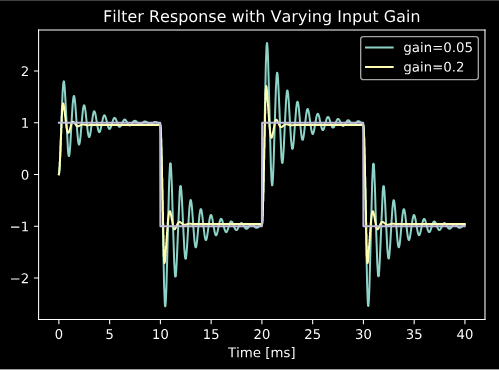
\includegraphics[width=3in]{../Pics/50-Hz_Response.png}
    \caption{\label{50hz}{\it Response of the nonlinear resonant lowpass
                            filter to a 50 Hz square wave with varying input gain.}}
\end{figure}
%
By tuning the input gain, we can attempt to match the response of an
arbitrary analog filter, either by tuning the parameters by ear
or using some form of numerical optimisation. Note that the choice
of base nonlinearities used by the nonlinear biquad will also play a
role in the accuracy of the model. For example, if the output of the
analog filter being modelled is asymmetric, then to accurately model
that filter, the nonlinear biquad must be constructed using an
asymmetric base nonlinearities.
\newline\newline
As an example, we can attempt to construct a naive model of Sallen-Key
lowpass filter, a commonly used analog filter structure. We describe this
as a naive model because we do not make any attempt to understand the physical
properties of the analog filter when constructing this model. We construct
a nonlinear biquad filter using $\tanh$ base nonlinearities, and design a
resonant lowpass filter with cutoff frequency $f_c = 1 \text{ kHz}$,
and $Q=10$, as well as a simulation of the corresponding Sallen-Key
filter using LTSpice. To accentuate the nonlinear behavior of the analog
filter, we choose $\pm 4 \text{ V}$ as the source voltages for the analog
filter circuit. We then compare the outputs of the two filters
for square waves at different frequencies, and use a simple staircase
optimisation scheme to find the input gain for the nonlinear biquad
that best matches the analog simulation. The results for the $250 \text{ Hz}$
square wave can be seen in \cref{SPICE}. While nonlinear biquad model
is not perfect, it does capture the damping effects of the analog filter
much more accurately than the corresponding linear filter, and can be greatly
improved with a more well-informed choice of base nonlinear functions, and
a more sophisticated optimisation scheme.
%
\begin{figure}[ht]
    \center
    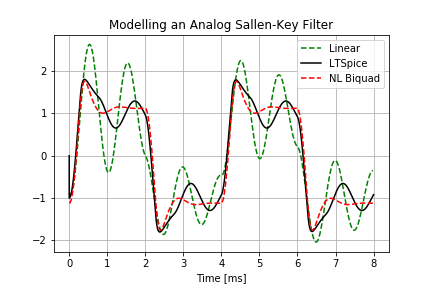
\includegraphics[width=3in]{../Pics/Spice-Compare.png}
    \caption{\label{SPICE}{\it Comparison between a linear resonant lowpass
                            filter, a resonant lowpass made with a nonlinear biquad
                            using a $\tanh$ clipper with input gain $0.283$,
                            and a SPICE simulation of a Sallen-Key lowpass.
                            All of the lowpass filters have $f_c=1$ kHz, and
                            $Q=10$. The input signal in each case is a $250$ Hz
                            square wave.}}
\end{figure}
%

\section{Conclusion}

In this paper, we have developed a structure for stable nonlinear biquad
filters. We have introduced the new architecture as a modification of the
Transposed Direct Form II filter form, and shown mathematically
how the changed architecture affects the pole locations depending on
the amplitude of the input signal. We have also derived constraints under
which the structure is guaranteed stable.
\newline\newline
As an example of the nonlinear biquad filter structure we have implemented
a nonlinear resonant lowpass filter, and shown that the poles respond to
the input as expected. We then show how the structure can be used to model
an analog filter, using a Sallen-Key lowpass filter as an example. Note
that while the nonlinear biquad structure can be used for analog modelling
it can also be used purely in the digital domain, as a tool for constructing
filters that sound more harmonically rich.
\newline\newline
To demonstrate this last point, we have also developed an open-source
audio plugin (VST, AU) implentation of the nonlinear biquad filter,
extending to several filter shapes, and several base nonlinearities.
The source code for the plugin implementation is available on
GitHub\footnote{\url{https://github.com/jatinchowdhury18/ComplexNonlinearities}}.
\newline\newline
Future research concerning nonlinear filtering will center around making a
more informed choice of base nonlinearities, focusing on both the desired
harmonic response of the filter, as well as physically meaningful base
nonlinearities for use in analog modelling.

%\newpage
\nocite{*}
\bibliographystyle{IEEEbib}
\bibliography{references}

\end{document}
